\UseRawInputEncoding
\documentclass[12pt,letterpaper]{article}
\usepackage{graphicx,textcomp}
\usepackage{natbib}
\usepackage{setspace}
\usepackage[margin=1in]{geometry}
\usepackage{color}
\usepackage[reqno]{amsmath}
\usepackage{amsthm}
\usepackage{fancyvrb}
\usepackage{amssymb,enumerate}
\usepackage[all]{xy}
\usepackage{endnotes}
\usepackage{lscape}
\newtheorem{com}{Comment}
\usepackage{float}
\usepackage{hyperref}
\newtheorem{lem} {Lemma}
\newtheorem{prop}{Proposition}
\newtheorem{thm}{Theorem}
\newtheorem{defn}{Definition}
\newtheorem{cor}{Corollary}
\newtheorem{obs}{Observation}
\usepackage[compact]{titlesec}
\usepackage{dcolumn}
\usepackage{tikz}
\usetikzlibrary{arrows}
\usepackage{multirow}
\usepackage{xcolor}
\newcolumntype{.}{D{.}{.}{-1}}
\newcolumntype{d}[1]{D{.}{.}{#1}}
\definecolor{light-gray}{gray}{0.65}
\usepackage{url}
\usepackage{listings}
\usepackage{color}

\definecolor{codegreen}{rgb}{0,0.6,0}
\definecolor{codegray}{rgb}{0.5,0.5,0.5}
\definecolor{codepurple}{rgb}{0.58,0,0.82}
\definecolor{backcolour}{rgb}{0.95,0.95,0.92}

\lstdefinestyle{mystyle}{
	backgroundcolor=\color{backcolour},   
	commentstyle=\color{codegreen},
	keywordstyle=\color{magenta},
	numberstyle=\tiny\color{codegray},
	stringstyle=\color{codepurple},
	basicstyle=\footnotesize,
	breakatwhitespace=false,         
	breaklines=true,                 
	captionpos=b,                    
	keepspaces=true,                 
	numbers=left,                    
	numbersep=5pt,                  
	showspaces=false,                
	showstringspaces=false,
	showtabs=false,                  
	tabsize=2
}
\lstset{style=mystyle}
\newcommand{\Sref}[1]{Section~\ref{#1}}
\newtheorem{hyp}{Hypothesis}

\title{Replication Project - Inclusion to Exclude: How Femonationalism Impacts Policy Preferences}
\date{April 1, 2026}
\author{Damaris Parasca}
\begin{document}
	\maketitle
	\section*{Original Paper}
		I replicated the paper, "Inclusion to Exclude: How Femonationalism Impacts Policy Preferences" by Sophie Mainz (2026), which explores how femonationalism affects the policy views (gender policies and immigration integration policies) of anti-immigration and pro-immigration citizens. \\[.2cm]
		Femonationalism generally refers to the concept introduced by Sara Farris (2017), defined as “the exploitation of feminist themes by nationalists and neoliberals in anti-Islam campaigns” and “the participation of certain feminists and femocrats in the stigmatization of Muslim men under the banner of gender equality”. Nevertheless, the chosen paper focuses on the general idea of selectively invoking gender equality to justify anti-immigrant policies by political actors. It also analyses the phenomenon away from the original European context studied by Farris (Italy, France and the Netherlands), moving it to the US. 
		\subsection*{Research Question}
		\textbf{How does femonationalism, defined as the selective invocation of gender equality to promote exclusionary anti-immigrant policies, affect citizens?} \\[.2cm]
		Specifically, it examines whether such rhetoric leads citizens to change their views on gender equality and immigrant integration, depending on their prior attitudes toward immigration.
		\subsection*{Research Contribution}
		The paper identifies and aims to fill several research gaps, making the following paramount contributions: 
		\begin{itemize}
			\item \textbf{Selective Illiberalism:} While previous research focused on how nativists adopt liberal views (selective liberalism), this paper shows that pro-immigration individuals can also shift toward illiberal stances (selective illiberalism) when faced with threat framing messages.
			\item \textbf{Expanded Scope:} It expands the study of femonationalism beyond European contexts and Muslim outgroups to the United States and Latino immigrants.
			\item \textbf{Conceptual Threat Distinction:} The paper introduces and tests a common distinction in femonationalist rhetoric: safety and value threats, and shows that such messages are embedded in partisan political contexts. 
		\end{itemize}
		\subsection*{Methodology}
		The study employs a survey experiment design, using fictive interview vignettes. The survey was taken by 3,118 U.S. citizens recruited via the Prolific platform, representative in terms of gender and party affiliation.The respondents were randomly assigned to a control group or one of four treatment groups that varied in two factors:
		\begin{itemize}
		\item Sender Partisanship: The message came from either a Republican or a Democratic senator.
		\item Threat Frame: The message depicted immigrants as either a value threat (threat to gender equality, emphasising the cultural otherness of migrants) or a safety threat (threat to women's safety and bodily integrity, drawing on notions of migrant women as victims of gender-based violence and patriarchal practices).
		\end{itemize} 
		Below are the texts of the utilised vignettes: 
			\begin{figure}[h!]\centering
			\caption{\footnotesize vignettes}
			\label{fig:vigs_1}
			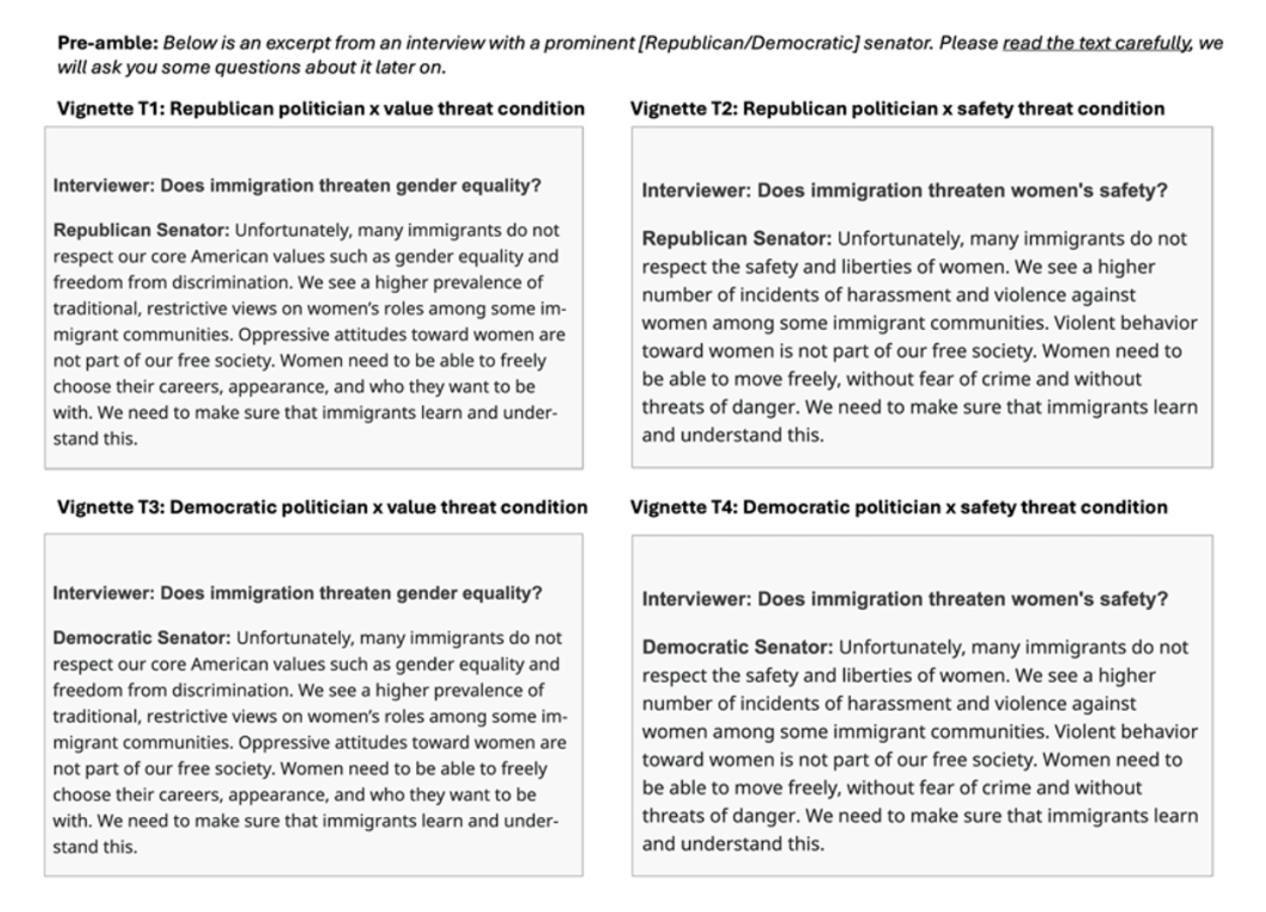
\includegraphics[width=.95\textwidth]{vignettes.png}
			\end{figure}
		\subsection*{Hypotheses}
		Elaborating on cognitive dissonance and identity theory, the paper puts forward two hypotheses: \\[.2cm]
			\indent \textbf{H1 (disidentification thesis):} Exposure to femonationalist speech by a politician from a party that represents a conservative immigration stance makes individuals with anti-immigration attitudes more supportive of gender equality policies. \\[0.2cm]
			\indent \textbf{H2 (liberal compromise thesis): }Exposure to femonationalist speech by a politician from a party that represents an inclusionary immigration stance makes individuals with pro-immigration attitudes more supportive of stricter integration policies.
		\vspace{.25cm}
		\subsection*{Variables of Interest}
		\underline{Explanatory variables:}
		\begin{itemize}
			\item immigration: prior immigration attitudes immigrants, measured on a 0–100 scale (0 - “Dislike a great deal” to 100 - “Like a great deal”); 
			\begin{figure} [h!]\centering
				\caption{\footnotesize immigration variable}
				\label{fig:vars_1}
				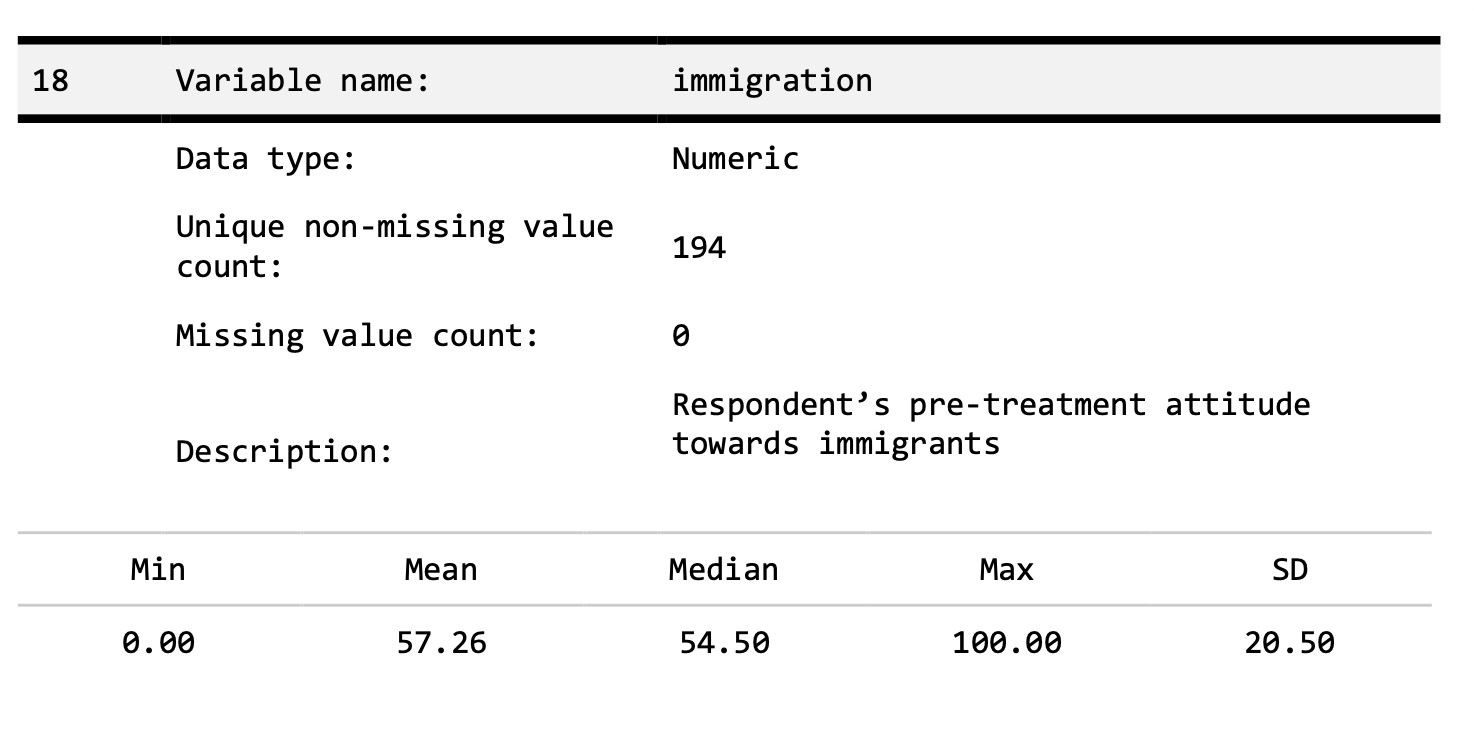
\includegraphics[width=.52\textwidth]{immigration.png}
			\end{figure}
			\item treatment: four types of treatment plus a control group. 
			\begin{figure}[h!]\centering
				\caption{\footnotesize treatment variable}
				\label{fig:vars_2}
				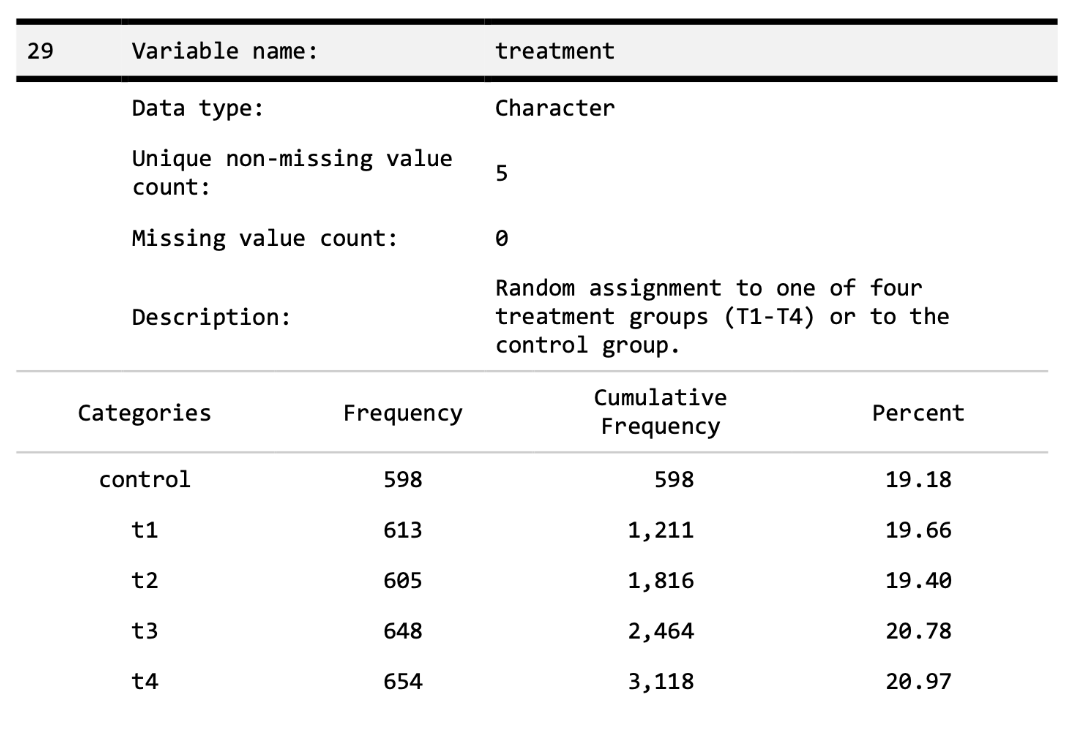
\includegraphics[width=.52\textwidth]{treatment.png}
			\end{figure}
		\end{itemize}
		\newpage
		\underline{Outcome variables: }
		\begin{itemize}
			\item support for gender education policies:
				\subitem support for school education on women's rights and equality; 
				\subitem support for education on sexual consent in public schools 
			\item support for  stricter integration demands:
				\subitem support for English language ability as a prerequisite for US citizenship; 
				\subitem support for classes on American societal norms and values.
			\begin{figure}[h!]\centering
				\caption{\footnotesize outcome variables}
				\label{fig:vars_3}
				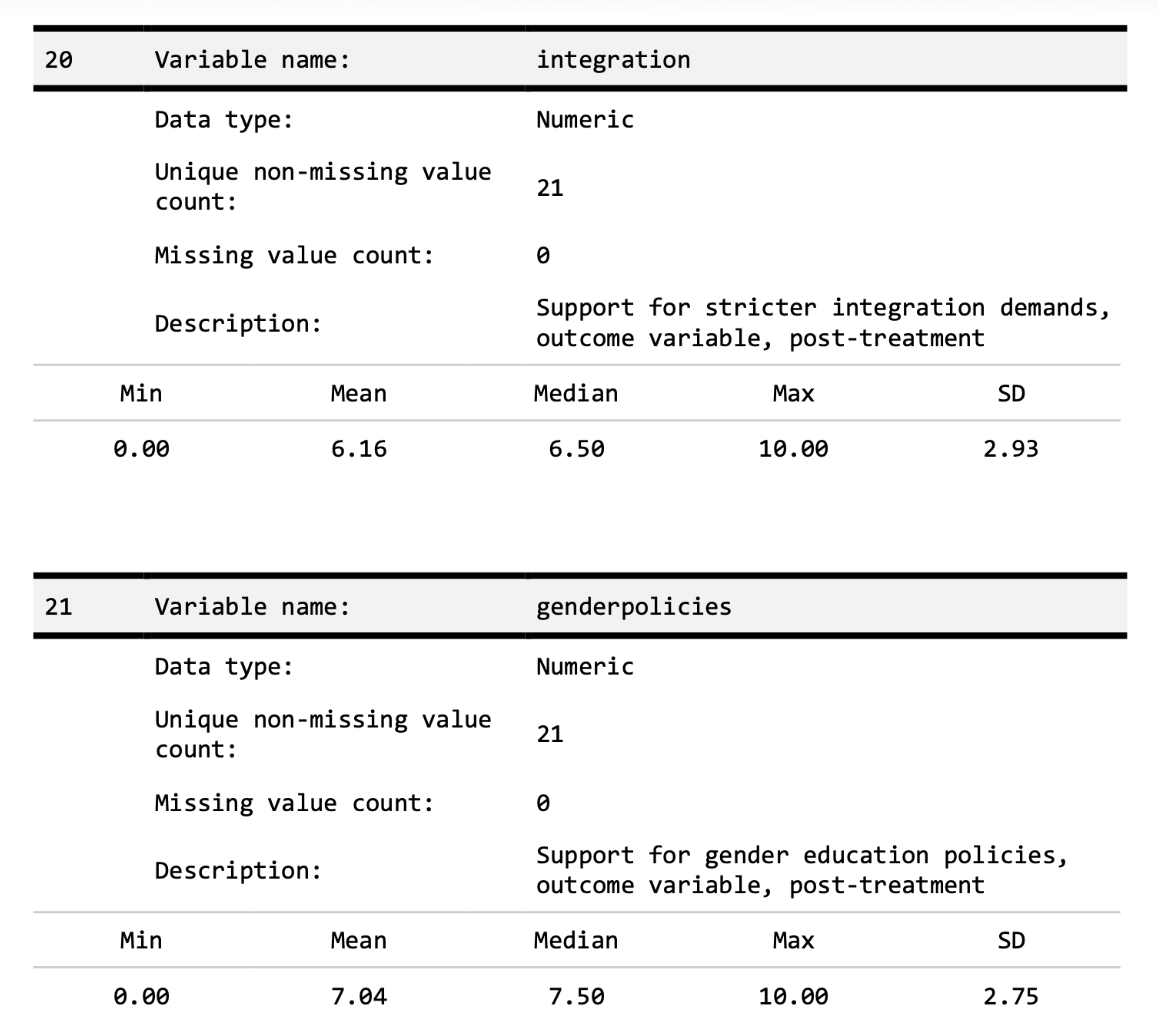
\includegraphics[width=.85\textwidth]{outcomes.png}
			\end{figure}
		\end{itemize}
		\newpage
		\subsection*{Model and Figures}
		\begin{table}[!htbp] \centering 
			\caption{} 
			\label{} 
			\begin{tabular}{@{\extracolsep{5pt}}lc} 
				\\[-1.8ex]\hline 
				\hline \\[-1.8ex] 
				& \multicolumn{1}{c}{\textit{Dependent variable:}} \\ 
				\cline{2-2} 
				\\[-1.8ex] & support for gender policies \\ 
				\hline \\[-1.8ex] 
				treatmentt1 & 0.905$^{**}$ \\ 
				& (0.420) \\ 
				& \\ 
				treatmentt2 & 1.211$^{***}$ \\ 
				& (0.424) \\ 
				& \\ 
				treatmentt3 & 0.506 \\ 
				& (0.411) \\ 
				& \\ 
				treatmentt4 & 0.490 \\ 
				& (0.413) \\ 
				& \\ 
				immigration & 0.062$^{***}$ \\ 
				& (0.005) \\ 
				& \\ 
				treatmentt1:immigration & $-$0.010 \\ 
				& (0.007) \\ 
				& \\ 
				treatmentt2:immigration & $-$0.015$^{**}$ \\ 
				& (0.007) \\ 
				& \\ 
				treatmentt3:immigration & $-$0.006 \\ 
				& (0.007) \\ 
				& \\ 
				treatmentt4:immigration & $-$0.002 \\ 
				& (0.007) \\ 
				& \\ 
				Constant & 3.230$^{***}$ \\ 
				& (0.292) \\ 
				& \\ 
				\hline \\[-1.8ex] 
				Observations & 3,118 \\ 
				R$^{2}$ & 0.179 \\ 
				Adjusted R$^{2}$ & 0.176 \\ 
				Residual Std. Error & 2.491 (df = 3108) \\ 
				F Statistic & 75.201$^{***}$ (df = 9; 3108) \\ 
				\hline 
				\hline \\[-1.8ex] 
				\textit{Note:}  & \multicolumn{1}{r}{$^{*}$p$<$0.1; $^{**}$p$<$0.05; $^{***}$p$<$0.01} \\ 
			\end{tabular} 
			\end{table}
				\noindent The author describes the figure below, as well as its implications: \\ [.2cm]
				"[the figure] presents the observed effect of femonationalist messages by a Republican politician on gender education policy preferences across all levels of immigration attitudes. (...). The upper panels plot the estimated regression slopes for treatment group 1, that is, respondents who received a message describing immigrants as threatening to gender equality, and for treatment group 2 who received a safety threat framing. The two lower panels present the Conditional Average Treatment Effects across the full range of prior immigration attitudes.\\[.2cm] (...) Those exposed to either treatment condition and with negative immigration attitudes display significantly higher support levels for gender education compared to their counterparts in the control group. This difference is slightly larger for the group that saw a safety threat message (T2) than for those who receive a value threat treatment (T1). The CATE between treatment and control is stronger with more adverse attitudes toward immigrants (...)."
		\begin{figure}[h!]
			\centering
			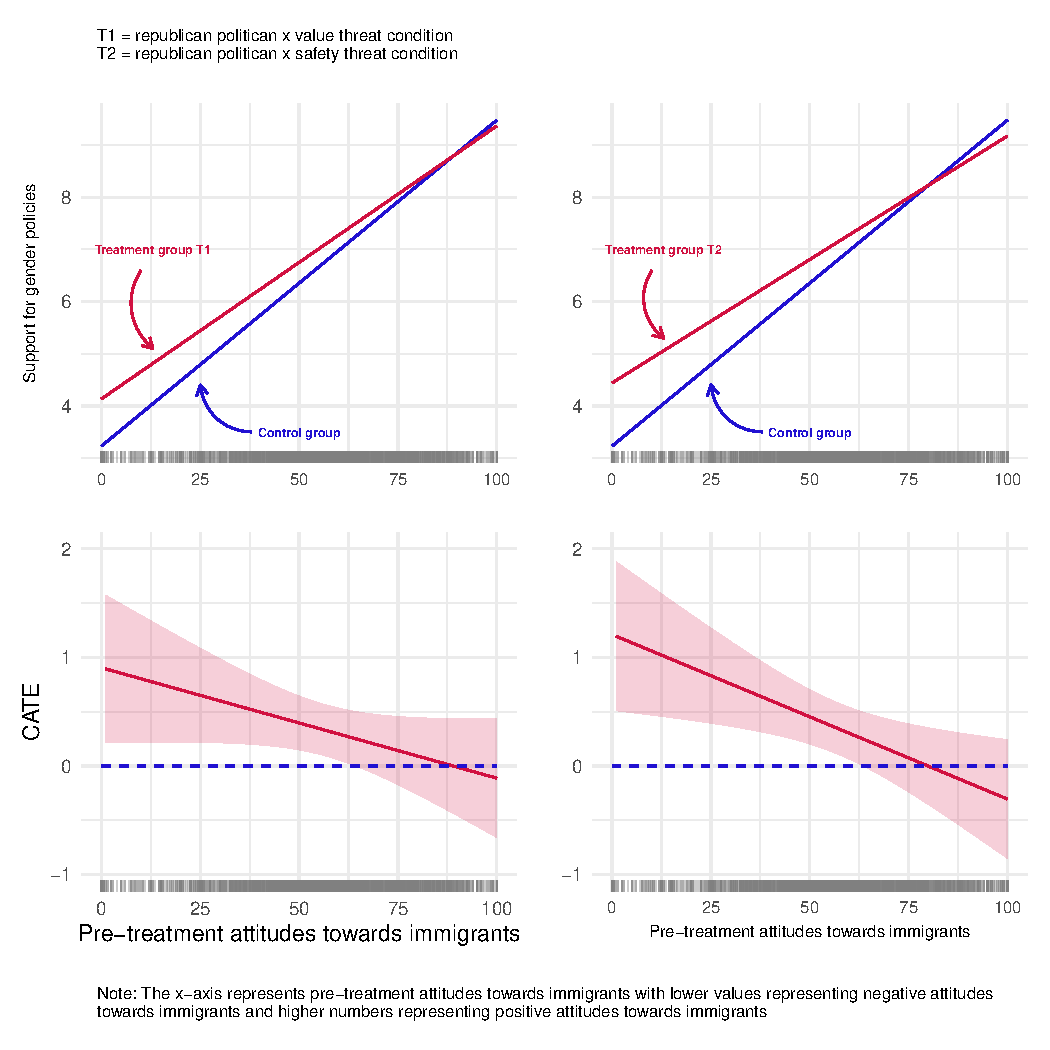
\includegraphics[width=0.75\textwidth]{joined_gender.pdf}
			\caption{\footnotesize Support for gender policies 1}
			\label{fig:plot_1}
 		\end{figure}
		\newpage
			\noindent The following figure is also described in the paper: \\[.2cm]
			''the hypothesized disidentification thesis (H1) is presented in more detail by stratifying the sample into pro- and anti-immigration respondents. The graph plots the mean support levels for gender education policies for all four treatment conditions and the control group for a dichotomous stratified sample relational to prior immigration attitudes.(...) \\[.2cm]
			Among anti-immigration respondents, all treated groups display higher support levels compared to the control group. The baseline mean of the control group is estimated at 5.36. Compared to that, immigration opponents who received a femonationalist claim by a Republican politician become significantly more inclined to favor gender education. For those who read a message describing immigrants as a threat to gender values this difference is .65 points (T1), while those receiving a safety-threat description increase their support levels by .83 points (T2). Messages by Democratic politicians do not show such strong effects on nativists: only treatment condition 4, has a small impact with a .44 point increase. This suggests that the receptiveness to femonationalist speech for people with averse immigration views is greater if the message comes from
			a like-minded source.''
			\begin{figure}[h!]
			\centering
			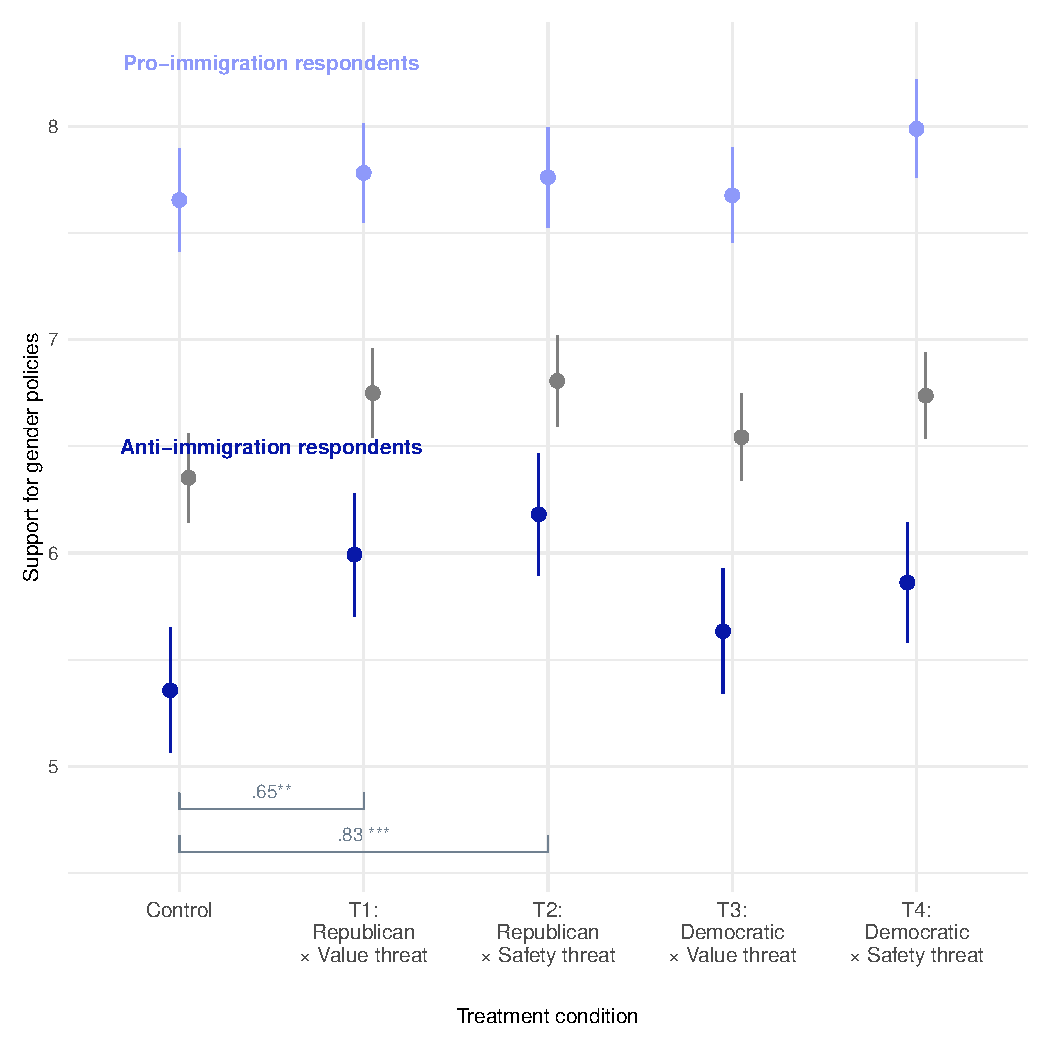
\includegraphics[width=0.8\textwidth]{support_gp.pdf}
			\caption{\footnotesize Support for gender policies 2}
			\label{fig:plot_2}
		\end{figure}
		\begin{table}[!htbp] \centering 
			\caption{} 
			\label{} 
			\begin{tabular}{@{\extracolsep{5pt}}lc} 
				\\[-1.8ex]\hline 
				\hline \\[-1.8ex] 
				& \multicolumn{1}{c}{\textit{Dependent variable:}} \\ 
				\cline{2-2} 
				\\[-1.8ex] &support for stricter integration policies \\ 
				\hline \\[-1.8ex] 
				treatmentt1 & $-$0.126 \\ 
				& (0.428) \\ 
				& \\ 
				treatmentt2 & 1.007$^{**}$ \\ 
				& (0.432) \\ 
				& \\ 
				treatmentt3 & $-$0.352 \\ 
				& (0.419) \\ 
				& \\ 
				treatmentt4 & 0.303 \\ 
				& (0.421) \\ 
				& \\ 
				immigration & $-$0.075$^{***}$ \\ 
				& (0.005) \\ 
				& \\ 
				treatmentt1:immigration & 0.009 \\ 
				& (0.007) \\ 
				& \\ 
				treatmentt2:immigration & $-$0.005 \\ 
				& (0.007) \\ 
				& \\ 
				treatmentt3:immigration & 0.013$^{*}$ \\ 
				& (0.007) \\ 
				& \\ 
				treatmentt4:immigration & 0.007 \\ 
				& (0.007) \\ 
				& \\ 
				Constant & 9.998$^{***}$ \\ 
				& (0.298) \\ 
				& \\ 
				\hline \\[-1.8ex] 
				Observations & 3,118 \\ 
				R$^{2}$ & 0.248 \\ 
				Adjusted R$^{2}$ & 0.246 \\ 
				Residual Std. Error & 2.542 (df = 3108) \\ 
				F Statistic & 113.904$^{***}$ (df = 9; 3108) \\ 
				\hline 
				\hline \\[-1.8ex] 
				\textit{Note:}  & \multicolumn{1}{r}{$^{*}$p$<$0.1; $^{**}$p$<$0.05; $^{***}$p$<$0.01} \\ 
			\end{tabular} 
		\end{table} 
		\newpage
		    \noindent Similarly, the author discusses the figure: \\[.2cm]
			''[the figure] summarizes the effects of femonationalist speech by a Democratic politician on integration preferences across all prior immigration attitudes. The top left panel depicts the estimated slopes for control and treatment group 3, those exposed to a description of immigrants as a threat to gender values. On the right is the respective plot for treatment group 4 who received a safety-threat message by a Democratic politician. Values on the y-axis reflect the scores on the combined measure for integration demands with lower values indicating disagreement to assimilationist policies, and higher values reflecting approval. The lower panels show the predicted CATEs of the two treatments across all levels of immigration attitudes. A negative control slope in the upper panels confirms that more liberal immigration views are associated with more inclusive
			stances on integration, dropping below a value of 4 for the highest 20
			percent. (...)  \\[.2cm]
			Those who received a femonationalist statement by a Democratic politician and share positive views toward immigrants deviate significantly from immigration advocates in the control group. This effect is slightly stronger for messages with a safety threat framing (T4) compared to value threat frames (T3), whilst this difference between treatment conditions is not significant.''
			\begin{figure}[h!]
			\centering
			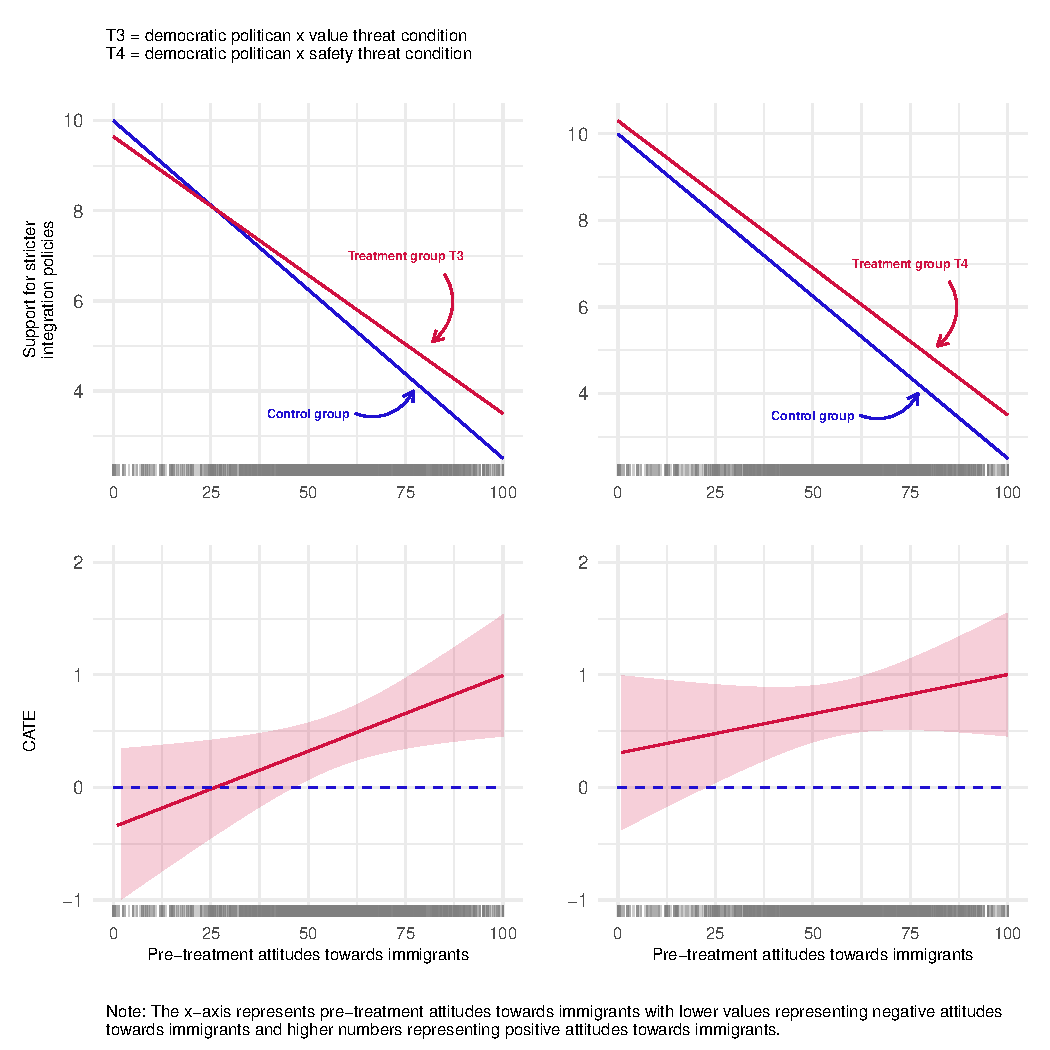
\includegraphics[width=0.72\textwidth]{joined_integ.pdf}
			\caption{\footnotesize Support for stricter integration policies 1}
			\label{fig:plot_3}
		\end{figure}
			\newpage
			\noindent Same with the figure below: \\[.2cm]
			''[it] presents a streamlined test of the liberal compromise mechanism by aggregating estimations of the CATE on the group level. The plot depicts mean support levels for stricter integration policies (0-10) among anti-immigration respondents and pro-immigration respondents. (...) Among immigration supporters, both T1 and T2 have a strong, significant effect on integration preferences (p <.01). The baseline mean of the control group is estimated at 4.69, suggesting disapproval of these policies. On average, this means that immigration supporters are more likely to approve of conditional naturalization and mandatory integration courses after exposure to a femonationalist message, while they are more likely to disapprove of such measures if they see no such message. The effect is substantively larger for immigration proponents exposed to a safety threat description than for those exposed to the value-based claim. Unlike expected, the effect of femonationalism on integration preferences among pro-immigration respondents is independent of the communicator’s party affiliation (...). \\[.2cm]
			Compared to pro-immigration respondents, nativist respondents score high on assimilationist integration demands regardless of the treatment condition, or whether they received no treatment. Only the safety threat argument by a Republican (T2) leads to a significant difference between treatment and control among nativists.'' 
			\begin{figure}[h!]
			\centering
			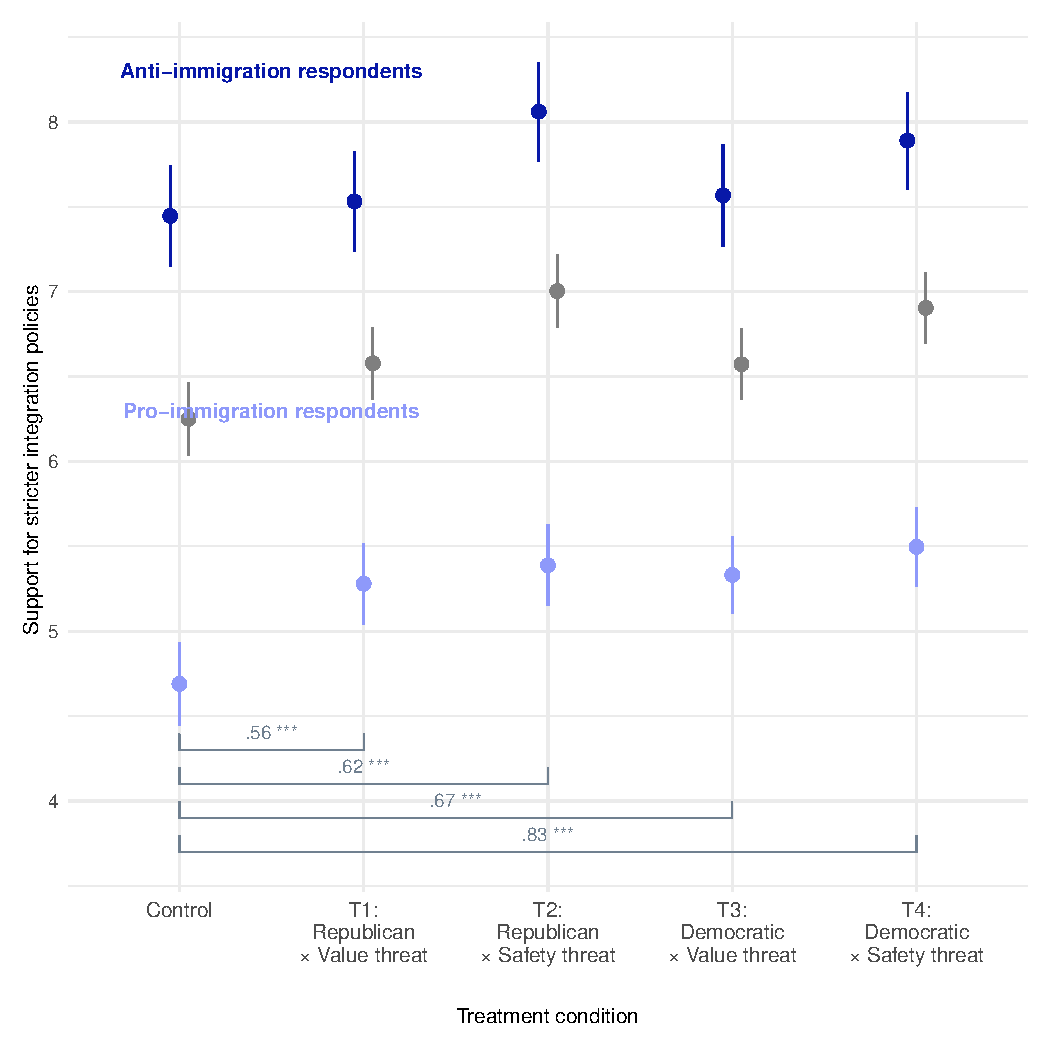
\includegraphics[width=0.7\textwidth]{int_attitudes.pdf}
			\caption{\footnotesize Support for stricter integration policies 2}
			\label{fig:plot_4}
		\end{figure}
		\newpage
			\noindent The last plot introduces a third interaction term, to examine gender-based variations in preferences adaptations. It finds that among nativists, men respond strongly to messages by a Republican politician, showing increased support for gender policies, while women and other genders are more responsive to the type of threat framing rather than the source. Among immigration supporters, both gender groups increase their support for stricter integration policies when exposed to femonationalist rhetoric, with particularly strong effects from messages by Democratic politicians.
			\begin{figure}[h!]
			\centering
			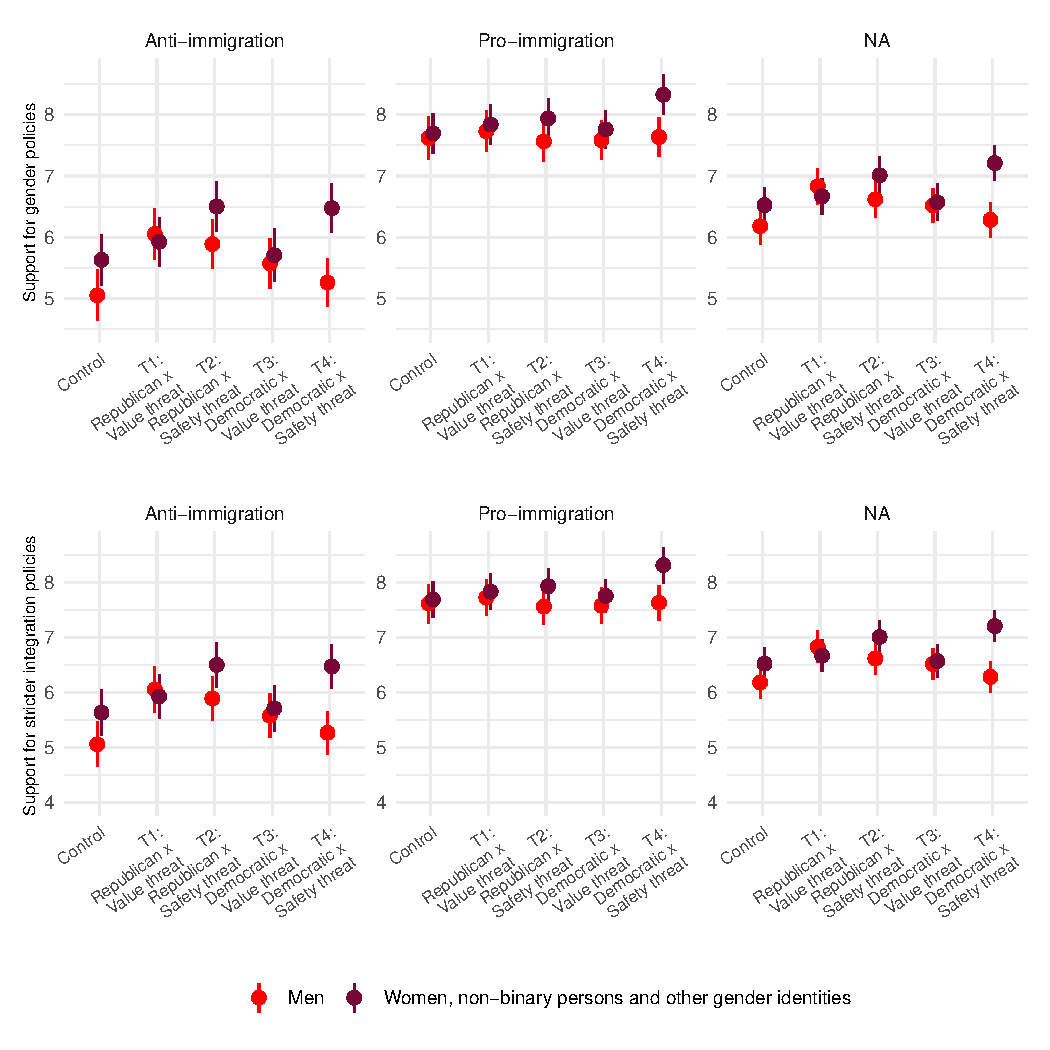
\includegraphics[width=0.9\textwidth]{gender_attitudes.pdf}
			\caption{\footnotesize Summary support plot}
			\label{fig:plot_5}
		\end{figure}
		\newpage
		\subsection*{Findings}
		\noindent Overall, the paper shows that femonationalist messages can shift policy preferences based on prior immigration attitudes,finding support for both its hypotheses. Among nativist individuals, such messages, especially from Republican messengers, increase support for more liberal gender policies, with stronger effects for more anti-immigration respondents (H1). Among pro-immigration individuals, femonationalist rhetoric, especially from Democratic messengers, increases support for stricter integration policies (H2). The last insight, presented in the plot above, is that the source and type of framing affect groups differently, with gender moderating these affects: men are more responsive to the message source, while other genders are more sensitive to framing.
		\vspace{.25cm}
		\subsection*{Replication Code}
		All the plots and models provided above have been replicated. Certain types of plots have been utilised twice (once for every outcome variable), so in that case I will only show the code once to avoid repetitiveness. I have selected parts I considered most interesting and relevant from the code. \\[.2cm]
		Code snippet for figure 5: 
		\lstinputlisting[language=R, firstline=45, lastline=69]{analysis_edited.R} 
		\lstinputlisting[language=R, firstline=145, lastline=165]{analysis_edited.R} 
		\vspace{.25cm}
		Code for snippet figure 6:
		\lstinputlisting[language=R, firstline=179, lastline=200]{analysis_edited.R}
		\newpage 
		\noindent Code for snippet figure 9: 
		\lstinputlisting[language=R, firstline=385, lastline=411]{analysis_edited.R}
		\lstinputlisting[language=R, firstline=434, lastline=438]{analysis_edited.R}
		\vspace{.25cm}
		Code for models: 
		\lstinputlisting[language=R, firstline=41, lastline=42]{analysis_edited.R} 
		\lstinputlisting[language=R, firstline=211, lastline=212]{analysis_edited.R} 
		\newpage
	\section*{My Twist}
		\subsection*{Argument}
		\begin{itemize}
			\item \textbf{Theoretical Argument} \\[.2cm]
		Existing literature typically frames femonationalism as a party-driven phenomenon (Fernandes et al., 2025). Moreover, femonationalism has primarily been theorized in a European context, particularly in relation to party rhetoric (Farris, 2017). Given that this paper focuses on the United States, a highly polarized political environment, I decided to extend this framework by examining whether partisan identity acts as a stronger filter for policy adaptation. 	I hypothesize that individuals adjust their policy preferences not only based on their prior attitudes toward immigration, but also according to their partisan identity.
			\item \textbf{Model Specification} \\[.2cm]
		To test this argument, I estimate the following model:
		\[
		\texttt{Policy Preference} \sim \texttt{Treatment} \times \texttt{Party} + \texttt{Immigration}
		\]
		Including immigration as a standalone covariate allows the model to account for baseline variation in policy preferences driven by prior immigration attitudes. The interaction between treatment and party captures how partisan identity conditions individuals' responses to the experimental treatments. This specification ensures that the interaction term isolates the effect of partisanship on treatment responses, rather than simply becoming a proxy for underlying immigration preferences.
			\item \textbf{Claim} \\[.2cm]
		I argue that partisanship operates as an independent moderator of treatment effects. Even when holding baseline immigration attitudes constant, partisan identity shapes how individuals respond to femonationalist messages. Finding support for this claim would suggest that femonationalism functions not only as an expression of nativist attitudes, but also as a mechanism of partisan alignment.
		\end{itemize}
		\subsection*{Code and Model}
		\lstinputlisting[language=R, firstline=494, lastline=521]{analysis_edited.R} 
		\lstinputlisting[language=R, firstline=527, lastline=558]{analysis_edited.R} 
		\begin{table}[!htbp] \centering 
			\caption{} 
			\label{} 
			\begin{tabular}{@{\extracolsep{5pt}}lc} 
				\\[-1.8ex]\hline 
				\hline \\[-1.8ex] 
				& \multicolumn{1}{c}{\textit{Dependent variable:}} \\ 
				\cline{2-2} 
				\\[-1.8ex] & support for gender policies \\ 
				\hline \\[-1.8ex] 
				treatmentt1 & 0.025 \\ 
				& (0.205) \\ 
				& \\ 
				treatmentt2 & $-$0.203 \\ 
				& (0.208) \\ 
				& \\ 
				treatmentt3 & $-$0.012 \\ 
				& (0.202) \\ 
				& \\ 
				treatmentt4 & 0.130 \\ 
				& (0.201) \\ 
				& \\ 
				party\_collapsedIndependent & $-$1.112$^{***}$ \\ 
				& (0.341) \\ 
				& \\ 
				party\_collapsedRepublican & $-$2.652$^{***}$ \\ 
				& (0.208) \\ 
				& \\ 
				immigration & 0.033$^{***}$ \\ 
				& (0.002) \\ 
				& \\ 
				treatmentt1:party\_collapsedRepublican & 0.705$^{**}$ \\ 
				& (0.285) \\ 
				& \\ 
				treatmentt2:party\_collapsedRepublican & 1.179$^{***}$ \\ 
				& (0.286) \\ 
				& \\ 
				treatmentt3:party\_collapsedRepublican & 0.568$^{**}$ \\ 
				& (0.281) \\ 
				& \\ 
				treatmentt4:party\_collapsedRepublican & 0.730$^{***}$ \\ 
				& (0.279) \\ 
				& \\ 
				Constant & 6.214$^{***}$ \\ 
				& (0.216) \\ 
				& \\ 
				\hline \\[-1.8ex] 
				\textit{Note:}  & \multicolumn{1}{r}{$^{*}$p$<$0.1; $^{**}$p$<$0.05; $^{***}$p$<$0.01} \\ 
			\end{tabular} 
		\end{table} 
		\begin{table}[!htbp] \centering 
			\caption{} 
			\label{} 
			\begin{tabular}{@{\extracolsep{5pt}}lc} 
				\\[-1.8ex]\hline 
				\hline \\[-1.8ex] 
				& \multicolumn{1}{c}{\textit{Dependent variable:}} \\ 
				\cline{2-2} 
				\\[-1.8ex] & support for stricter integration policies \\ 
				\hline \\[-1.8ex] 
				treatmentt1 & 0.688$^{***}$ \\ 
				& (0.213) \\ 
				& \\ 
				treatmentt2 & 0.853$^{***}$ \\ 
				& (0.216) \\ 
				& \\ 
				treatmentt3 & 0.843$^{***}$ \\ 
				& (0.210) \\ 
				& \\ 
				treatmentt4 & 1.111$^{***}$ \\ 
				& (0.209) \\ 
				& \\ 
				party\_collapsedIndependent & 0.879$^{**}$ \\ 
				& (0.354) \\ 
				& \\ 
				party\_collapsedRepublican & 2.308$^{***}$ \\ 
				& (0.216) \\ 
				& \\ 
				immigration & $-$0.050$^{***}$ \\ 
				& (0.002) \\ 
				& \\ 
				treatmentt1:party\_collapsedRepublican & $-$0.623$^{**}$ \\ 
				& (0.296) \\ 
				& \\ 
				treatmentt2:party\_collapsedRepublican & $-$0.343 \\ 
				& (0.297) \\ 
				& \\ 
				treatmentt3:party\_collapsedRepublican & $-$1.023$^{***}$ \\ 
				& (0.291) \\ 
				& \\ 
				treatmentt4:party\_collapsedRepublican & $-$0.797$^{***}$ \\ 
				& (0.289) \\ 
				& \\ 
				Constant & 7.442$^{***}$ \\ 
				& (0.224) \\ 
				& \\ 
				\hline \\[-1.8ex] 
				\textit{Note:}  & \multicolumn{1}{r}{$^{*}$p$<$0.1; $^{**}$p$<$0.05; $^{***}$p$<$0.01} \\ 
			\end{tabular} 
		\end{table} 
		\subsection*{Figures and Tests}
		\begin{figure}[h!]
		\centering
		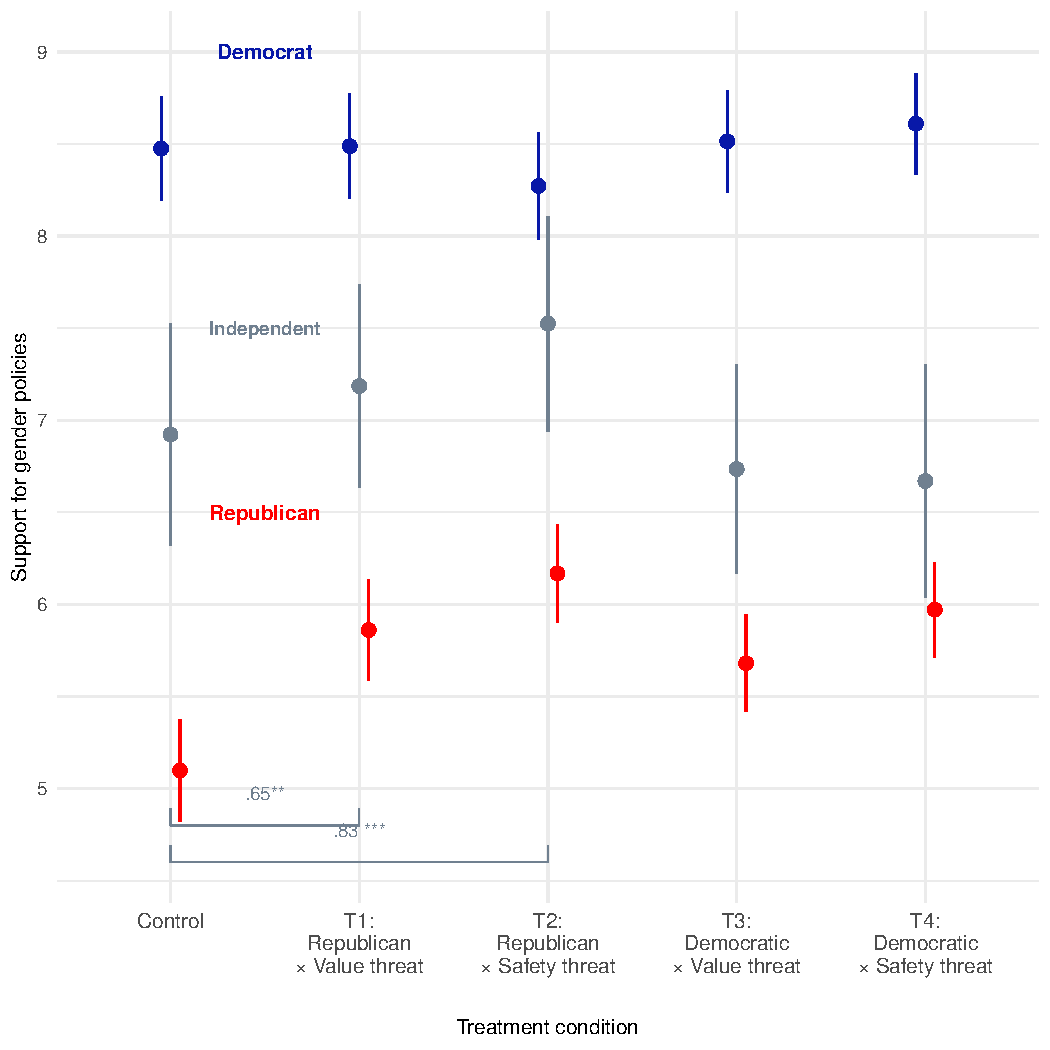
\includegraphics[width=0.55\textwidth]{support_gp_twist.pdf}
		\caption{\footnotesize Twist plot - gender policies}
		\label{fig:plot_6}
		\end{figure}
		\begin{figure}[h!]
			\centering
			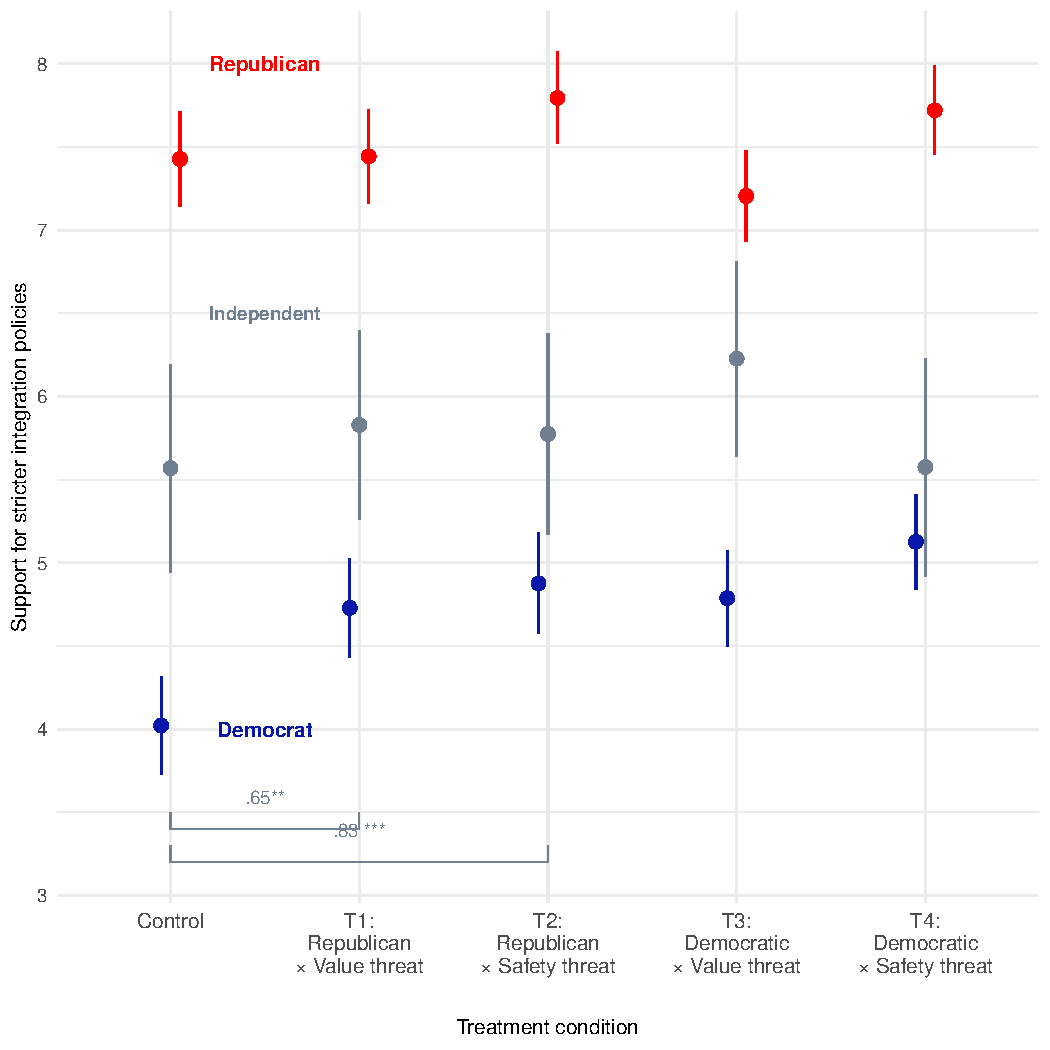
\includegraphics[width=0.55\textwidth]{support_ip_twist.pdf}
			\caption{\footnotesize Twist plot - integration policies}
			\label{fig:plot_7}
		\end{figure}
		\newpage
			\begin{verbatim}
			Analysis of Variance Table
			
			Model 1: genderpolicies ~ treatment * immigration
			Model 2: genderpolicies ~ treatment * party_collapsed + immigration
			Res.Df   RSS Df Sum of Sq      F    Pr(>F)    
			1   3100 19251                                  
			2   3094 16985  6    2265.4 68.777 < 2.2e-16 ***
			---
			Signif. codes:  0 ‘***’ 0.001 ‘**’ 0.01 ‘*’ 0.05 ‘.’ 0.1 ‘ ’ 1
		\end{verbatim}
		\begin{verbatim}
			Analysis of Variance Table
			
			Model 1: integration ~ treatment * immigration
			Model 2: integration ~ treatment * party_collapsed + immigration
			Res.Df   RSS Df Sum of Sq      F    Pr(>F)    
			1   3100 20029                                  
			2   3094 18317  6    1712.5 48.213 < 2.2e-16 ***
			---
			Signif. codes:  0 ‘***’ 0.001 ‘**’ 0.01 ‘*’ 0.05 ‘.’ 0.1 ‘ ’ 1
		\end{verbatim}			
		\subsection*{Twist Findings}
		\begin{itemize}
			\item \textbf{F-test:} \\[.2cm]
				The statistical justification for the twist is provided by the F-tests above, which compare the performance of the original models used in the paper with the expanded partisan interaction model. For both the gender policy and the integration policy, the twist model provides an improvement in model fit. The F-statistics are very high and the p-values fall well below the 0.05 threshold, indicating that the twist models explain more variability in the outcome than the original models.
			\item \textbf{Gender policy:} \\[.2cm]
				While the baseline support for gender policies is significantly lower for Republicans compared to Democrats (reference category), the treatments add meaningful nuance. All four treatments show positive and statistically significant effects for Republicans, with t2 (Republican x safety threat) being the strongest effect. Interestingly, while the effect is not as strong when the message is delivered by a Democrat senator, it is still non-negligible and statistically significant. While the Democrats’ views on gender equality remain relatively stable across treatments, Republicans are mobilised toward more progressive gender policy stances, with little importance given to the messenger. 
			\item \textbf{Integration policy:} \\[.2cm]
				In contrast to the effect seen in gender policies, the results for integration policy seem to significantly impact both partisan groups. For Democrats, all treatments show significant positive coefficients, suggesting that they are pushed toward stricter integration policy stances. However, for Republicans, the interaction terms are consistently negative, moderating their stances in support of strict integration policies. It is still important to consider that Republicans start at a much higher (2.3 points higher) baseline of support for strict integration, but the treatments have the opposite effect of intensifying their stance. Interestingly, Democrats' support for stricter integration policies increases no matter the messenger, meanwhile Republicans' support decreases significantly more when the messenger is a Democrat. 
			\item \textbf{Immigration:} \\[.2cm]
			In both models, the immigration variable remains highly statistically significant. In the gender policy model, pro-immigrant views are associated with higher support for the policies, and in the integration model, they are correlated with lower support for strict policies. The effects of the variable remaining significant, along with the partisan interactions, confirm that partisanship provides a separate layer to the analysis. Partisanship is an important dimension that should be considered when studying femonationalism and the effect of political communication. 
		\end{itemize}
		\subsection*{Conclusion}
		The twist adds additional theoretical insight to the paper, which is easiest to understand in the context of the paper’s hypotheses:
		\begin{itemize}
			\item \textbf{H1 (Disidentification Thesis):} Exposure to femonationalist speech by a politician from a party that represents a conservative immigration stance makes individuals with anti-immigration attitudes more supportive of gender equality policies.
			\item \textbf{H2 (Liberal Compromise Thesis):} Exposure to femonationalist speech by a politician from a party that represents an inclusionary immigration stance makes individuals with pro-immigration attitudes more supportive of stricter integration policies.
	\end{itemize}
		\noindent In relation to H1, my extension shows that exposure to femonationalist speech, regardless of the speaker’s partisan affiliation, leads Republicans to become more supportive of gender equality policies (all interaction terms are statistically significant). For H2, Democrats exposed to femonationalist speech, irrespective of the source, become more supportive of stricter integration policies. In contrast, Republicans tend to either maintain their baseline preferences or, particularly when exposed to a Democratic source, slightly reduce their support for such policies. \\[.2cm]
		Overall, these findings suggest that individuals with the same partisan affiliation respond in similar ways to femonationalist messages, largely independent of the speaker’s party. This implies that partisan identity operates more through in-group predispositions than through sensitivity to the identity of the message source. In other words, people do not primarily react to who delivers the message, but rather process the message through their existing partisan lens. \\[.2cm]
		An additional insight is that partisan identity appears to partially override immigration attitudes as a moderator, indicating that political identity may be a stronger organising principle in highly polarised contexts like the United States. At the same time, the consistent strength of safety-threat framing across groups suggests that certain types of messaging have stronger persuasive power, regardless of partisan alignment. \\[.2cm]
		All in all, while the original hypotheses emphasise the interaction between immigration attitudes and message source, this extension highlights that partisan identity plays an independent and potentially dominant role in shaping responses to femonationalist rhetoric.
		\newpage
		\begin{thebibliography}{}
			\bibitem{farris2017}
			Farris, S. R. (2017).
			\textit{In the name of women’s rights: The rise of femonationalism}.
			Duke University Press.
			https://doi.org/10.1215/9780822372929
			\bibitem{fernandes2025}
			Fernandes, J., Meguid, B. M., \& Weeks, A. C. (2025).
			\textit{Thinly veiled: The use of femonationalist speech in European parliaments}
			(Working paper). SSRN.
			https://doi.org/10.2139/ssrn.5107245
			\bibitem{mainz2026}
			Mainz, S. (2026).
			\textit{Inclusion to exclude: How femonationalism impacts policy preferences}.
			Political Science Research and Methods.
			https://doi.org/10.1017/psrm.2025.10068
		\end{thebibliography}
\end{document}